%!TEX program = xelate
%%%%%%%%%%%%%%%%%%%%%%%%%%%%%%%%%%%%%%%%%
% Modified By Orcuslc, 2016-9-21
% Modified for Assignments
% http://github.com/orcuslc
%
% Wilson Resume/CV
% Structure Specification File
% Version 1.0 (22/1/2015)
%
% This file has been downloaded from:
% http://www.LaTeXTemplates.com
%
% License:
% CC BY-NC-SA 3.0 (http://creativecommons.org/licenses/by-nc-sa/3.0/)
%
%%%%%%%%%%%%%%%%%%%%%%%%%%%%%%%%%%%%%%%%%

%----------------------------------------------------------------------------------------
%	PACKAGES AND OTHER DOCUMENT CONFIGURATIONS
%----------------------------------------------------------------------------------------
\documentclass[10pt]{article}

\usepackage{listings}
\usepackage{xcolor}
\usepackage{amsmath,amsthm,amssymb}
\usepackage{epstopdf}
\usepackage{graphicx}
\usepackage{clrscode3e}

\DeclareGraphicsExtensions{.eps,.ps,.jpg,.bmp}


\usepackage[a4paper, hmargin=25mm, vmargin=30mm, top=20mm]{geometry} % Use A4 paper and set margins

\usepackage{fancyhdr} % Customize the header and footer

\usepackage{lastpage} % Required for calculating the number of pages in the document

\usepackage{hyperref} % Colors for links, text and headings

\setcounter{secnumdepth}{0} % Suppress section numbering

%\usepackage[proportional,scaled=1.064]{erewhon} % Use the Erewhon font
%\usepackage[erewhon,vvarbb,bigdelims]{newtxmath} % Use the Erewhon font
\usepackage[utf8]{inputenc} % Required for inputting international characters
\usepackage[T1]{fontenc} % Output font encoding for international characters

\usepackage{fontspec} % Required for specification of custom fonts
\setmainfont[Path = ./fonts/,
Extension = .otf,
BoldFont = Erewhon-Bold,
ItalicFont = Erewhon-Italic,
BoldItalicFont = Erewhon-BoldItalic,
SmallCapsFeatures = {Letters = SmallCaps}
]{Erewhon-Regular}

\usepackage{color} % Required for custom colors
\definecolor{slateblue}{rgb}{0.17,0.22,0.34}

\usepackage{sectsty} % Allows customization of titles
\sectionfont{\color{slateblue}} % Color section titles

\fancypagestyle{plain}{\fancyhf{}\cfoot{\thepage\ of \pageref{LastPage}}} % Define a custom page style
\pagestyle{plain} % Use the custom page style through the document
\renewcommand{\headrulewidth}{0pt} % Disable the default header rule
\renewcommand{\footrulewidth}{0pt} % Disable the default footer rule

\setlength\parindent{0pt} % Stop paragraph indentation

% Non-indenting itemize
\newenvironment{itemize-noindent}
{\setlength{\leftmargini}{0em}\begin{itemize}}
{\end{itemize}}

% Text width for tabbing environments
\newlength{\smallertextwidth}
\setlength{\smallertextwidth}{\textwidth}
\addtolength{\smallertextwidth}{-2cm}

\newcommand{\sqbullet}{~\vrule height .8ex width .6ex depth -.05ex} % Custom square bullet point 


\newcommand{\tbf}[1]{\textbf{#1}}
\newcommand{\tit}[1]{\textit{#1}}
\newcommand{\mbb}[1]{\mathbb{#1}}
\newcommand{\blue}[1]{\color{blue}{#1}}
\newcommand{\red}[1]{\color{red}{#1}}
\newcommand{\sblue}[1]{\color{slateblue}{#1}}
\newcommand{\n}{\\[5pt]}
\newcommand{\tr}{^\top}
\newcommand{\vt}[1]{
\Vert #1 \Vert
}
\newcommand{\bra}[5]{
#1=\left\{
\begin{aligned}
#2 ,&\quad #4 \\
#3 ,&\quad #5
\end{aligned}
\right.
}

\renewcommand{\title}[2] {
{\Huge{\color{slateblue}\textbf{#1}}}
\hfill
\LARGE{\color{slateblue}\textbf{#2}} \\[10pt]
\large{\color{slateblue}\textbf{Chuan Lu, 13300180056, chuanlu13@fudan.edu.cn}} \\[1mm]
\rule{\textwidth}{0.5mm}
}

\newcommand{\problem}[2] {
\vspace{20pt}
\LARGE{\color{slateblue}\textbf{Problem #1.}}
\vspace{2mm}
#2 \\[10pt]
}

\renewcommand{\proof}[2] {
\large{\color{slateblue}\textit{\textbf{#1.}}}
#2 \qed \\[3mm]
}

\newcommand{\solution}[2] {
\large{\color{slateblue}\textit{\textbf{#1.}}}
#2 \\[3mm]
}


\newcommand{\algorithm}[2] {
\begin{codebox}
\Procname{$\proc{Algorithm #1}$}
#2
\end{codebox}
}

\newcommand{\refgroup}[1] {
\LARGE{\color{slateblue}\textbf{Reference}} 
\begin{tabbing}
\hspace{5mm} \= \kill
#1
\end{tabbing}
}

\newcommand{\reference}[1] {
\sqbullet \ \  \large{#1} \\
}
% \newcommand{\solution}[2] {
% \LARGE{\color{slateblue}\textit{#1}}
% \ #2 \qed
% }

% \newenvironment{problem}[2][Problem]{\begin{trivlist}
% \item[\hskip \labelsep {\bfseries #1}\hskip \labelsep {\bfseries #2.}]}{\end{trivlist}}
\usepackage{epstopdf}
\usepackage{graphics}
\usepackage{subfig}
\usepackage{listings}
\lstset{
  breaklines=true,
  xleftmargin=25pt,
  xrightmargin=25pt,
  aboveskip=0pt,
  belowskip=10pt,
  basicstyle=\ttfamily,
  showstringspaces=false,
  frame=ltrb,
  tabsize=4,
  numbers=left,
  numberstyle=\small,
  numbersep=8pt,
  morekeywords={*, factorial, sum, erlang},
  keywordstyle=\color{blue!70}, commentstyle=\color{red!50!green!50!blue!50},
}
\DeclareGraphicsExtensions{.eps,.ps,.jpg,.bmp}

\begin{document}

\title{Numerical Analysis \\ Assignment 5}
\date{\today}
\author{Chuan Lu}

\maketitle

\problem{1}{Problem 2.21, Page 121}
\solution{Solution}{
According to Theorem 2.7, we should choose $c$ so as to have $|g'(\alpha)| < 1$. Thus
$$
|g'(\alpha)| = |1+cf'(\alpha)| < 1.
$$
So $c$ satisfies $-2 < cf'(\alpha) < 0$. For a good rate of convergence, pick $c$ s.t. $cf'(\alpha) \sim 0$.
}

\problem{2}{Problem 2.24, Page 121}
\solution{Solution}{
\textbf{(a)} 
$$
g(x) = -16+6x+\frac{12}{x}.
$$
Thus $g'(2) = 3 > 1.$ So the iteration does not converge. 

\textbf{(b)}
$$
g(x) = \frac{2}{3}x+\frac{1}{x^2}.
$$
Thus $g'(3^{\frac{1}{3}}) = \frac{2}{3}-2\alpha^{-3} = 0$. So the iteration converges. Since
$$
\begin{aligned}
\lim_{n\to\infty}\frac{\alpha-x_{n+1}}{(\alpha-x_n)^2} &= \lim_{n\to\infty}\frac{-2x_n^3+3\alpha x_n^2-3}{3x_n^2(\alpha-x_n)^2} = \lim_{x_n\to\alpha}\frac{-2x_n^3+3\alpha x_n^2-3}{3x_n^2(\alpha-x_n)^2}\\
&= \lim_{x_n\to\alpha}\frac{-6x_n^2+6\alpha x_n}{6x_n(\alpha-x_n)^2-6x_n^2(\alpha-x_n)} = \lim_{x_n\to\alpha}\frac{1}{\alpha-2x_n} \\
&= -\frac{1}{\alpha}.
\end{aligned}
$$
We know the iteration is second-order convergent.

\textbf{(c)}
$$
g(x) = \frac{12}{1+x}.
$$
Thus $g'(\alpha) = -\frac{3}{4}$, so the iteration converges. Since
$$
\lim_{n\to\infty}\frac{\alpha-x_{n+1}}{\alpha-x_n} = \frac{(1+x_n)\alpha-12}{(1+x_n)(\alpha-x_n)} = \frac{\alpha}{\alpha-2x_n-1} = -\frac{3}{4},
$$
We know the iteration is linear convergence, and the rate is $\frac{3}{4}$.
}

\problem{3}{Problem 2.28, Page 122}
\solution{Proof}{
Assume $f(x) = (x-\alpha)h(x), ~h(\alpha) \ne 0$. Then
$$
\begin{aligned}
g(x) &= x - \frac{f(x)}{D(x)} = x-\frac{(x-\alpha)^2h^2(x)}{(x-\alpha)(h(x)+1)h((x-\alpha)h(x)+x)-(x-\alpha)h(x)} \\
&= x - \frac{(x-\alpha)h^2(x)}{(h(x)+1)h((x-\alpha)h(x)+x)-h(x)}.
\end{aligned}
$$
Thus 
$$
\begin{aligned}
g'(\alpha) &= \left.1-\frac{(h^2(x)+2(x-\alpha)h(x)h'(x))((h(x)+1)h((x-\alpha)h(x)+x)-h(x)) - (x-\alpha)M}{((h(x)+1)h((x-\alpha)h(x)+x)-h(x))^2}\right|_{x=\alpha} \\
&= 1-\frac{h^4(\alpha)}{h^4(\alpha)} = 0.
\end{aligned}
$$
And we can know that $g''(\alpha)\ne 0$. Accoding to Theorem 2.8, this iteration is a second-order method.
}

\problem{4}{Problem 2.48, Page 126}
\solution{Proof}{
According to the continuity of $\lVert\cdot\rVert_{\infty}$, we can find an $\epsilon$ and a closed set $B(\alpha, \delta)$, s.t. $\forall x\in B(\alpha, \delta)$, $\lVert G(x)\rVert_{\infty} \le 1-\epsilon$. Then $\forall x_0 \in B = B(\alpha, \delta)$,
$$
\lVert \alpha-x_{n+1}\rVert = \lVert g(\alpha)-g(x_n)\rVert = \lVert G(\xi)\rVert \cdot \lVert \alpha-x_n\rVert \le (1-\epsilon) \lVert \alpha-x_n\rVert \le (1-\epsilon)^n \lVert \alpha-x_0\rVert.
$$
Thus $\lVert \alpha-x_{n+1}\rVert \to 0, ~t\to\infty$. So the iteration converges to $\alpha$. And since $g(B) \subset B$ according to that $\lVert\alpha-g(x)\rVert < \lVert\alpha-x\rVert$, and $\max \lVert G(x)\rVert < 1$, we know that it satisfies the condition of Theorem 2.9.
}

\problem{5}{Problem 2.50, Page 127}
\solution{Solution}{
The code and result are as follows;(In fact)
}
\lstinputlisting[language = MATLAB]{Newton.m}
\lstinputlisting[language = MATLAB]{prob50.m}
\begin{lstlisting}[language = MATLAB]
>> prob50
   1.600000000000000   1.200000000000000
   1.581250000000000   1.225000000000000
   1.581138833992095   1.224744897959184
\end{lstlisting}

\problem{6}{Problem 2.51, Page 127}
\solution{Solution}{
We just use the code of Newton's method from Problem 2.50, and the executive script is as follows;
}
\lstinputlisting[language = MATLAB]{prob51.m}
\solution{Result}{
The result is shown in the following table \ref{Table 1}, and the convergence speed shown in \ref{Graph 1}. From the result we know that different initial values may lead to convergence to different roots, while when the iteration comes to very close to the root, the convergence order is first-order.
}
\begin{table}[!htb]
\centering
\begin{tabular}{|c|c|c|c|}
\hline
Initial Point & Convergence & Result & Number of iterates \\
\hline
(1.2, 2.5) & Yes & (1.336355248159268, 1.754234729131226) & 11 \\
\hline
(-2, 2.5) & Yes & (1.336355247361990, 1.754234726236878) & 19 \\
\hline
(-1.2, -2.5) & Yes & (1.336355235838950, 1.754234684404958) & 24 \\
\hline
(2, -2.5) & Yes & (2.998365352785336, 0.148430977265564) & 9 \\
\hline
\end{tabular}
\caption{The result of convergence and iteration count.}
\label{Table 1}
\end{table}

\begin{figure}[!htb]
\centering
\begin{minipage}{0.45\textwidth}
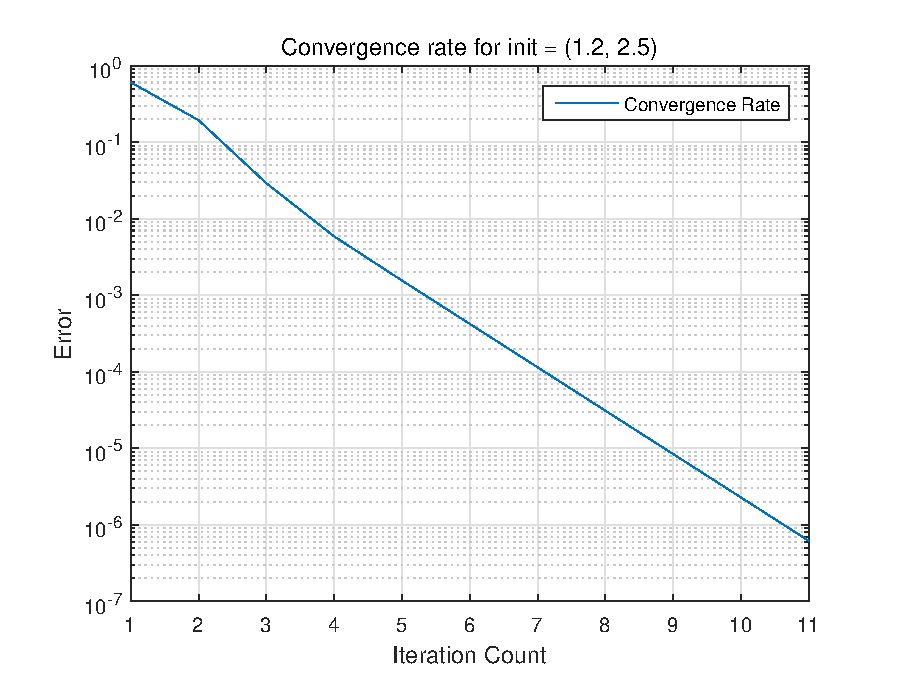
\includegraphics[width = \textwidth]{res1.eps}
\end{minipage}
\begin{minipage}{0.45\textwidth}
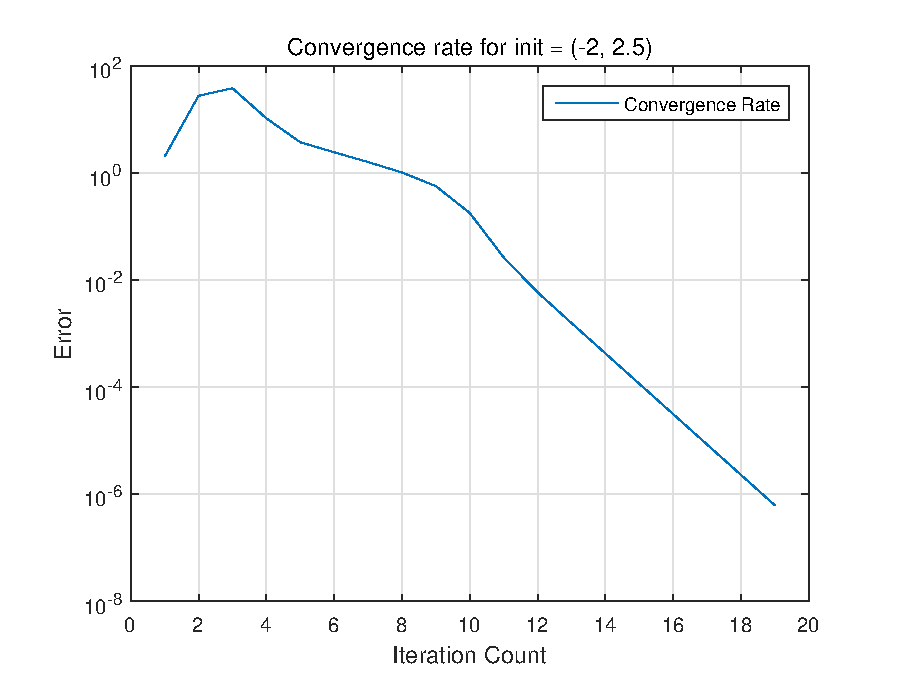
\includegraphics[width = \textwidth]{res2.eps}
\end{minipage} \\
\begin{minipage}{0.45\textwidth}
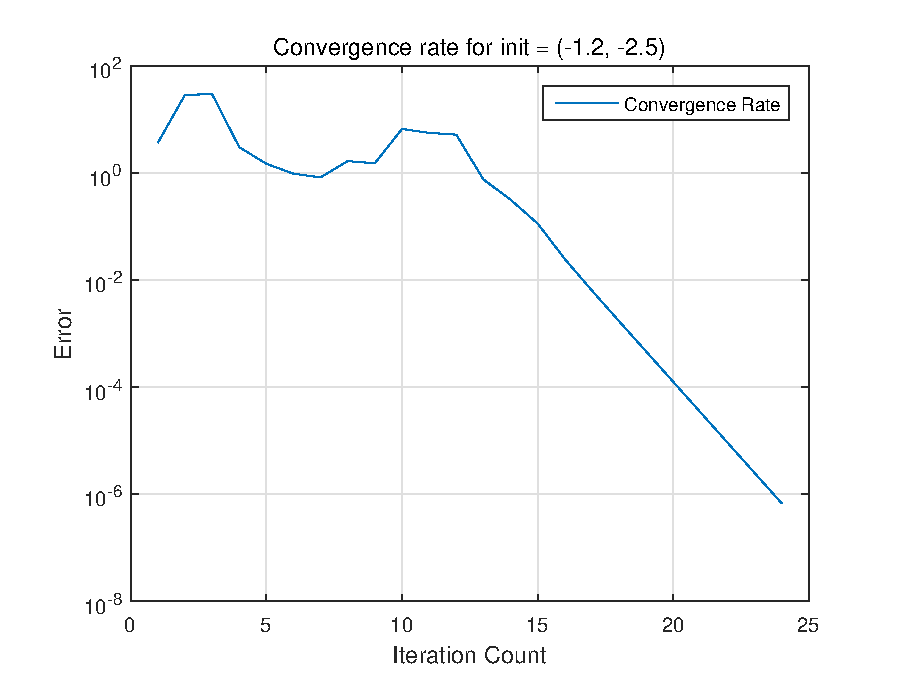
\includegraphics[width = \textwidth]{res3.eps}
\end{minipage}
\begin{minipage}{0.45\textwidth}
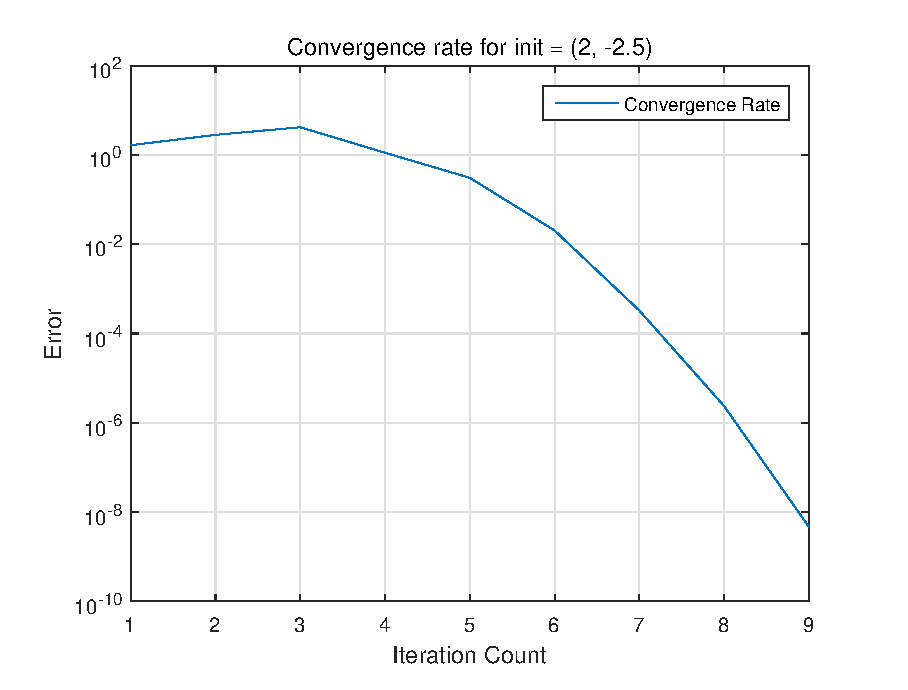
\includegraphics[width = \textwidth]{res4.eps}
\end{minipage}
\caption{Convergence Order}
\label{Figure 1}
\end{figure}
\end{document}